\documentclass[12pt,letterpaper]{report}
\usepackage[top=1in, bottom=1in, left=1in, right=1in]{geometry}
\geometry{bindingoffset=0.2in}
\usepackage{pgfplots}
\usepackage{subcaption}
\usepackage{hyperref}
\pgfplotsset{compat=newest} 
\pgfplotsset{plot coordinates/math parser=false} 
\newlength\figureheight 
\newlength\figurewidth 
\begin{document}

\begin{figure}
A
\caption{turds}\label{fig:samplepath_paths}
\end{figure}



\clearpage
\begin{figure}%
\centering%
\setlength\figureheight{0.16\linewidth}%
\setlength\figurewidth{0.4\linewidth}%
\begin{subfigure}[b]{\linewidth}%
  \centering%
  %\tikzsetnextfilename{samplepath_cts_bookvalue}%
  % This file was created by matlab2tikz.
%
%The latest updates can be retrieved from
%  http://www.mathworks.com/matlabcentral/fileexchange/22022-matlab2tikz-matlab2tikz
%where you can also make suggestions and rate matlab2tikz.
%
\begin{tikzpicture}[trim axis left, trim axis right]

\begin{axis}[%
width=\figurewidth,
height=\figureheight,
at={(0\figurewidth,0\figureheight)},
scale only axis,
separate axis lines,
every outer x axis line/.append style={black},
every x tick label/.append style={font=\color{black}},
xtick = {10.97,10.98,10.99,11},
xmin=10.975,
xmax=11,
every outer y axis line/.append style={black},
every y tick label/.append style={font=\color{black}},
ymin=1.56,
ymax=1.72,
axis background/.style={fill=white}
]
\addplot [color=black,solid,line width=2.0pt,forget plot]
  table[row sep=crcr]{%
10.975	1.62135739067691\\
10.9752777777778	1.62135739067691\\
10.9755555555556	1.62135739067691\\
10.9758333333333	1.62135739067691\\
10.9761111111111	1.62135739067691\\
10.9763888888889	1.62135739067691\\
10.9766666666667	1.62135739067691\\
10.9769444444444	1.6013573906769\\
10.9772222222222	1.6013573906769\\
10.9775	1.58420236875733\\
10.9777777777778	1.58420236875733\\
10.9780555555556	1.56949457134348\\
10.9783333333333	1.56949457134348\\
10.9786111111111	1.56949457134348\\
10.9788888888889	1.56949457134348\\
10.9791666666667	1.60579404440273\\
10.9794444444444	1.60579404440273\\
10.9797222222222	1.60579404440273\\
10.98	1.60579404440273\\
10.9802777777778	1.60579404440273\\
10.9805555555556	1.60579404440273\\
10.9808333333333	1.60579404440273\\
10.9811111111111	1.64294906632227\\
10.9813888888889	1.64294906632227\\
10.9816666666667	1.64294906632227\\
10.9819444444444	1.64294906632227\\
10.9822222222222	1.64294906632227\\
10.9825	1.64294906632227\\
10.9827777777778	1.64294906632227\\
10.9830555555556	1.64294906632227\\
10.9833333333333	1.63294906632228\\
10.9836111111111	1.63294906632228\\
10.9838888888889	1.63294906632228\\
10.9841666666667	1.63294906632228\\
10.9844444444444	1.63294906632228\\
10.9847222222222	1.63294906632228\\
10.985	1.63294906632228\\
10.9852777777778	1.63294906632228\\
10.9855555555556	1.62664959326301\\
10.9858333333333	1.636649593263\\
10.9861111111111	1.636649593263\\
10.9863888888889	1.636649593263\\
10.9866666666667	1.636649593263\\
10.9869444444444	1.636649593263\\
10.9872222222222	1.636649593263\\
10.9875	1.636649593263\\
10.9877777777778	1.636649593263\\
10.9880555555556	1.636649593263\\
10.9883333333333	1.636649593263\\
10.9886111111111	1.63926150765013\\
10.9888888888889	1.63926150765013\\
10.9891666666667	1.63926150765013\\
10.9894444444444	1.63926150765013\\
10.9897222222222	1.63926150765013\\
10.99	1.63926150765013\\
10.9902777777778	1.63926150765013\\
10.9905555555556	1.63926150765013\\
10.9908333333333	1.63926150765013\\
10.9911111111111	1.63926150765013\\
10.9913888888889	1.65038174658721\\
10.9916666666667	1.65038174658721\\
10.9919444444444	1.65038174658721\\
10.9922222222222	1.65038174658721\\
10.9925	1.65038174658721\\
10.9927777777778	1.65038174658721\\
10.9930555555556	1.65038174658721\\
10.9933333333333	1.66038174658721\\
10.9936111111111	1.66038174658721\\
10.9938888888889	1.66038174658721\\
10.9941666666667	1.66038174658721\\
10.9944444444444	1.6703817465872\\
10.9947222222222	1.66038174658721\\
10.995	1.66038174658721\\
10.9952777777778	1.66038174658721\\
10.9955555555556	1.66038174658721\\
10.9958333333333	1.66038174658721\\
10.9961111111111	1.66038174658721\\
10.9963888888889	1.66512562991656\\
10.9966666666667	1.66512562991656\\
10.9969444444444	1.66512562991656\\
10.9972222222222	1.66512562991656\\
10.9975	1.66512562991656\\
10.9977777777778	1.67522571701728\\
10.9980555555556	1.69773749116025\\
10.9983333333333	1.70271710009541\\
10.9986111111111	1.70271710009541\\
10.9988888888889	1.6827171000954\\
10.9991666666667	1.6827171000954\\
10.9994444444444	1.6827171000954\\
10.9997222222222	1.6827171000954\\
11	1.6827171000954\\
};
\end{axis}
\end{tikzpicture}%
%
  \hspace{1.5cm}%
  %\tikzsetnextfilename{samplepath_cts_inventory}%
  % This file was created by matlab2tikz.
%
%The latest updates can be retrieved from
%  http://www.mathworks.com/matlabcentral/fileexchange/22022-matlab2tikz-matlab2tikz
%where you can also make suggestions and rate matlab2tikz.
%
\begin{tikzpicture}[trim axis left, trim axis right]

\begin{axis}[%
width=\figurewidth,
height=\figureheight,
at={(0\figurewidth,0\figureheight)},
scale only axis,
separate axis lines,
every outer x axis line/.append style={black},
every x tick label/.append style={font=\color{black}},
xmin=10.975,
xmax=11,
every outer y axis line/.append style={black},
every y tick label/.append style={font=\color{black}},
ymin=1,
ymax=7,
axis background/.style={fill=white}
]
\addplot [color=black,solid,line width=2.0pt,forget plot]
  table[row sep=crcr]{%
10.975	2\\
10.9752777777778	2\\
10.9755555555556	2\\
10.9758333333333	2\\
10.9761111111111	2\\
10.9763888888889	2\\
10.9766666666667	2\\
10.9769444444444	3\\
10.9772222222222	3\\
10.9775	4\\
10.9777777777778	4\\
10.9780555555556	5\\
10.9783333333333	5\\
10.9786111111111	5\\
10.9788888888889	5\\
10.9791666666667	4\\
10.9794444444444	4\\
10.9797222222222	4\\
10.98	4\\
10.9802777777778	4\\
10.9805555555556	4\\
10.9808333333333	4\\
10.9811111111111	3\\
10.9813888888889	3\\
10.9816666666667	3\\
10.9819444444444	3\\
10.9822222222222	3\\
10.9825	3\\
10.9827777777778	3\\
10.9830555555556	3\\
10.9833333333333	4\\
10.9836111111111	4\\
10.9838888888889	4\\
10.9841666666667	4\\
10.9844444444444	4\\
10.9847222222222	4\\
10.985	4\\
10.9852777777778	4\\
10.9855555555556	5\\
10.9858333333333	4\\
10.9861111111111	4\\
10.9863888888889	4\\
10.9866666666667	4\\
10.9869444444444	4\\
10.9872222222222	4\\
10.9875	4\\
10.9877777777778	4\\
10.9880555555556	5\\
10.9883333333333	5\\
10.9886111111111	6\\
10.9888888888889	6\\
10.9891666666667	6\\
10.9894444444444	6\\
10.9897222222222	6\\
10.99	6\\
10.9902777777778	6\\
10.9905555555556	6\\
10.9908333333333	6\\
10.9911111111111	3\\
10.9913888888889	2\\
10.9916666666667	2\\
10.9919444444444	2\\
10.9922222222222	2\\
10.9925	2\\
10.9927777777778	2\\
10.9930555555556	2\\
10.9933333333333	3\\
10.9936111111111	2\\
10.9938888888889	2\\
10.9941666666667	2\\
10.9944444444444	1\\
10.9947222222222	2\\
10.995	3\\
10.9952777777778	3\\
10.9955555555556	3\\
10.9958333333333	3\\
10.9961111111111	3\\
10.9963888888889	4\\
10.9966666666667	4\\
10.9969444444444	4\\
10.9972222222222	4\\
10.9975	4\\
10.9977777777778	3\\
10.9980555555556	2\\
10.9983333333333	2\\
10.9986111111111	2\\
10.9988888888889	3\\
10.9991666666667	3\\
10.9994444444444	3\\
10.9997222222222	3\\
11	3\\
};
\end{axis}
\end{tikzpicture}%
%
  \caption{Continuous Time}%
\end{subfigure}\\%
\vspace{1cm}%
\begin{subfigure}[b]{\linewidth}%
  \centering
  %\tikzsetnextfilename{samplepath_dscr_bookvalue}%
  % This file was created by matlab2tikz.
%
%The latest updates can be retrieved from
%  http://www.mathworks.com/matlabcentral/fileexchange/22022-matlab2tikz-matlab2tikz
%where you can also make suggestions and rate matlab2tikz.
%
\begin{tikzpicture}[trim axis left, trim axis right]

\begin{axis}[%
width=\figurewidth,
height=\figureheight,
at={(0\figurewidth,0\figureheight)},
scale only axis,
separate axis lines,
every outer x axis line/.append style={black},
every x tick label/.append style={font=\color{black}},
xtick = {10.97,10.98,10.99,11},
xmin=10.975,
xmax=11,
every outer y axis line/.append style={black},
every y tick label/.append style={font=\color{black}},
ymin=2.22,
ymax=2.29,
axis background/.style={fill=white}
]
\addplot [color=black,solid,line width=2.0pt,forget plot]
  table[row sep=crcr]{%
10.975	2.27140001455481\\
10.9752777777778	2.27140001455481\\
10.9755555555556	2.27140001455481\\
10.9758333333333	2.27140001455481\\
10.9761111111111	2.27140001455481\\
10.9763888888889	2.27140001455481\\
10.9766666666667	2.27140001455481\\
10.9769444444444	2.25571186515924\\
10.9772222222222	2.25571186515924\\
10.9775	2.24009762920537\\
10.9777777777778	2.24009762920537\\
10.9780555555556	2.24009762920537\\
10.9783333333333	2.24009762920537\\
10.9786111111111	2.24009762920537\\
10.9788888888889	2.24009762920537\\
10.9791666666667	2.24009762920537\\
10.9794444444444	2.24009762920537\\
10.9797222222222	2.24009762920537\\
10.98	2.24009762920537\\
10.9802777777778	2.22918770726608\\
10.9805555555556	2.22918770726608\\
10.9808333333333	2.22918770726608\\
10.9811111111111	2.26473439318914\\
10.9813888888889	2.24574941841536\\
10.9816666666667	2.24574941841536\\
10.9819444444444	2.24574941841536\\
10.9822222222222	2.24574941841536\\
10.9825	2.24574941841536\\
10.9827777777778	2.24574941841536\\
10.9830555555556	2.24574941841536\\
10.9833333333333	2.23802678373983\\
10.9836111111111	2.23802678373983\\
10.9838888888889	2.23802678373983\\
10.9841666666667	2.23255755255633\\
10.9844444444444	2.23255755255633\\
10.9847222222222	2.23255755255633\\
10.985	2.23255755255633\\
10.9852777777778	2.23255755255633\\
10.9855555555556	2.22710906192009\\
10.9858333333333	2.22710906192009\\
10.9861111111111	2.22710906192009\\
10.9863888888889	2.22168141919798\\
10.9866666666667	2.22168141919798\\
10.9869444444444	2.22168141919798\\
10.9872222222222	2.22168141919798\\
10.9875	2.22168141919798\\
10.9877777777778	2.22168141919798\\
10.9880555555556	2.22168141919792\\
10.9883333333333	2.22168141919792\\
10.9886111111111	2.22404308918556\\
10.9888888888889	2.22404308918556\\
10.9891666666667	2.22404308918556\\
10.9894444444444	2.22404308918556\\
10.9897222222222	2.22404308918556\\
10.99	2.22404308918556\\
10.9902777777778	2.22404308918556\\
10.9905555555556	2.22404308918556\\
10.9908333333333	2.22404308918556\\
10.9911111111111	2.22404308918556\\
10.9913888888889	2.22522861167261\\
10.9916666666667	2.22522861167261\\
10.9919444444444	2.22522861167261\\
10.9922222222222	2.22522861167261\\
10.9925	2.22522861167261\\
10.9927777777778	2.22522861167261\\
10.9930555555556	2.22522861167261\\
10.9933333333333	2.2352286116726\\
10.9936111111111	2.22951614259546\\
10.9938888888889	2.22951614259546\\
10.9941666666667	2.22951614259546\\
10.9944444444444	2.22951614259546\\
10.9947222222222	2.22951614259546\\
10.995	2.23419887278612\\
10.9952777777778	2.23515848561965\\
10.9955555555556	2.23515848561965\\
10.9958333333333	2.23515848561965\\
10.9961111111111	2.23515848561965\\
10.9963888888889	2.23515848561965\\
10.9966666666667	2.23515848561965\\
10.9969444444444	2.23515848561965\\
10.9972222222222	2.23515848561965\\
10.9975	2.25277459230335\\
10.9977777777778	2.25277459230335\\
10.9980555555556	2.24277459230336\\
10.9983333333333	2.28346494645052\\
10.9986111111111	2.28346494645052\\
10.9988888888889	2.26346494645054\\
10.9991666666667	2.26346494645054\\
10.9994444444444	2.26346494645054\\
10.9997222222222	2.26346494645054\\
11	2.26346494645054\\
};
\end{axis}
\end{tikzpicture}%
%
  \hspace{1.5cm}%
  %\tikzsetnextfilename{samplepath_dscr_inventory}%
  % This file was created by matlab2tikz.
%
%The latest updates can be retrieved from
%  http://www.mathworks.com/matlabcentral/fileexchange/22022-matlab2tikz-matlab2tikz
%where you can also make suggestions and rate matlab2tikz.
%
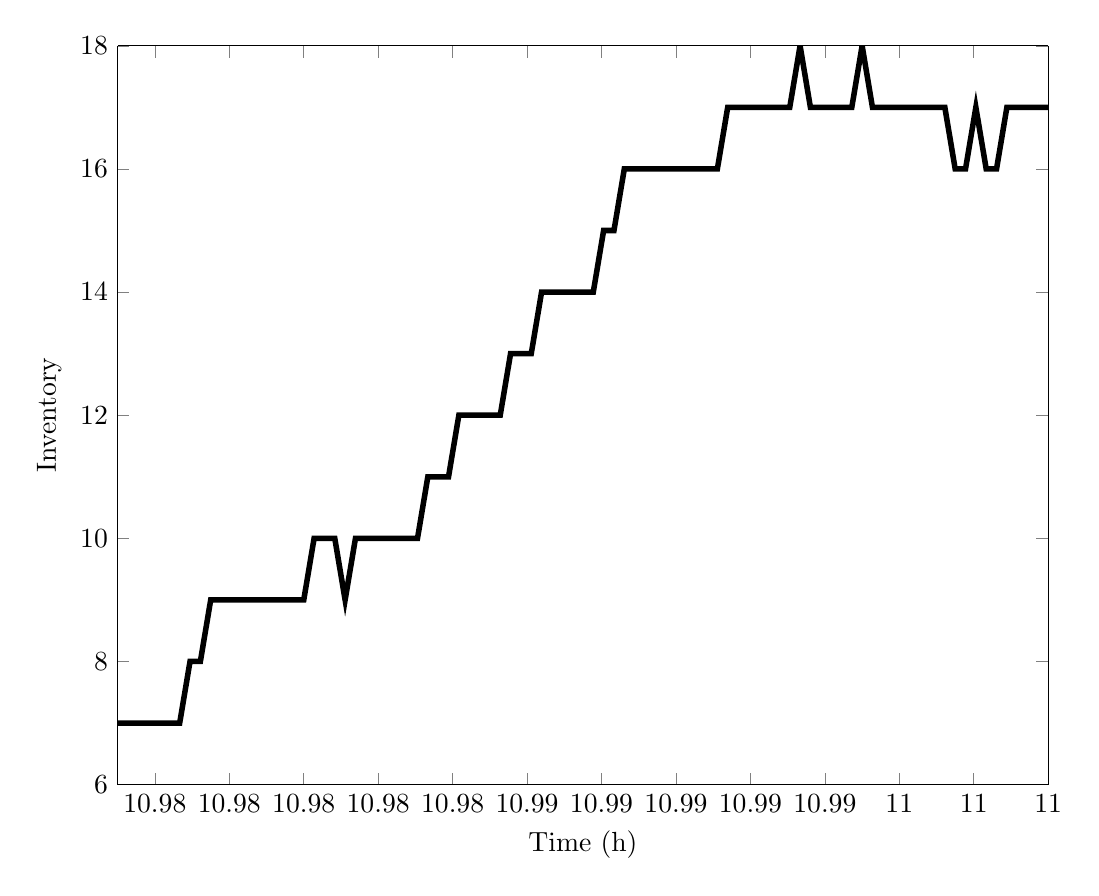
\begin{tikzpicture}

\begin{axis}[%
width=4.653in,
height=3.694in,
at={(0.978in,0.622in)},
scale only axis,
separate axis lines,
every outer x axis line/.append style={black},
every x tick label/.append style={font=\color{black}},
xmin=10.975,
xmax=11,
xlabel={Time (h)},
every outer y axis line/.append style={black},
every y tick label/.append style={font=\color{black}},
ymin=6,
ymax=18,
ylabel={Inventory},
axis background/.style={fill=white}
]
\addplot [color=black,solid,line width=2.0pt,forget plot]
  table[row sep=crcr]{%
10.975	7\\
10.9752777777778	7\\
10.9755555555556	7\\
10.9758333333333	7\\
10.9761111111111	7\\
10.9763888888889	7\\
10.9766666666667	7\\
10.9769444444444	8\\
10.9772222222222	8\\
10.9775	9\\
10.9777777777778	9\\
10.9780555555556	9\\
10.9783333333333	9\\
10.9786111111111	9\\
10.9788888888889	9\\
10.9791666666667	9\\
10.9794444444444	9\\
10.9797222222222	9\\
10.98	9\\
10.9802777777778	10\\
10.9805555555556	10\\
10.9808333333333	10\\
10.9811111111111	9\\
10.9813888888889	10\\
10.9816666666667	10\\
10.9819444444444	10\\
10.9822222222222	10\\
10.9825	10\\
10.9827777777778	10\\
10.9830555555556	10\\
10.9833333333333	11\\
10.9836111111111	11\\
10.9838888888889	11\\
10.9841666666667	12\\
10.9844444444444	12\\
10.9847222222222	12\\
10.985	12\\
10.9852777777778	12\\
10.9855555555556	13\\
10.9858333333333	13\\
10.9861111111111	13\\
10.9863888888889	14\\
10.9866666666667	14\\
10.9869444444444	14\\
10.9872222222222	14\\
10.9875	14\\
10.9877777777778	14\\
10.9880555555556	15\\
10.9883333333333	15\\
10.9886111111111	16\\
10.9888888888889	16\\
10.9891666666667	16\\
10.9894444444444	16\\
10.9897222222222	16\\
10.99	16\\
10.9902777777778	16\\
10.9905555555556	16\\
10.9908333333333	16\\
10.9911111111111	16\\
10.9913888888889	17\\
10.9916666666667	17\\
10.9919444444444	17\\
10.9922222222222	17\\
10.9925	17\\
10.9927777777778	17\\
10.9930555555556	17\\
10.9933333333333	18\\
10.9936111111111	17\\
10.9938888888889	17\\
10.9941666666667	17\\
10.9944444444444	17\\
10.9947222222222	17\\
10.995	18\\
10.9952777777778	17\\
10.9955555555556	17\\
10.9958333333333	17\\
10.9961111111111	17\\
10.9963888888889	17\\
10.9966666666667	17\\
10.9969444444444	17\\
10.9972222222222	17\\
10.9975	16\\
10.9977777777778	16\\
10.9980555555556	17\\
10.9983333333333	16\\
10.9986111111111	16\\
10.9988888888889	17\\
10.9991666666667	17\\
10.9994444444444	17\\
10.9997222222222	17\\
11	17\\
};
\end{axis}
\end{tikzpicture}%%
  \caption{Discrete Time}%
\end{subfigure}\\%
\vspace{1cm}%
\begin{subfigure}[b]{\linewidth}%
  \centering%
  %\tikzsetnextfilename{samplepath_cts_nFPC_bookvalue}%
  % This file was created by matlab2tikz.
%
%The latest updates can be retrieved from
%  http://www.mathworks.com/matlabcentral/fileexchange/22022-matlab2tikz-matlab2tikz
%where you can also make suggestions and rate matlab2tikz.
%
\begin{tikzpicture}[trim axis left, trim axis right]

\begin{axis}[%
width=\figurewidth,
height=\figureheight,
at={(0\figurewidth,0\figureheight)},
scale only axis,
separate axis lines,
every outer x axis line/.append style={black},
every x tick label/.append style={font=\color{black}},
xmin=10.975,
xmax=11,
every outer y axis line/.append style={black},
every y tick label/.append style={font=\color{black}},
ymin=-7.4,
ymax=-7.05,
axis background/.style={fill=white}
]
\addplot [color=black,solid,line width=2.0pt,forget plot]
  table[row sep=crcr]{%
10.975	-7.07965620945679\\
10.9752777777778	-7.07965620945679\\
10.9755555555556	-7.07965620945679\\
10.9758333333333	-7.07965620945679\\
10.9761111111111	-7.07965620945679\\
10.9763888888889	-7.07965620945679\\
10.9766666666667	-7.07965620945679\\
10.9769444444444	-7.09965620945678\\
10.9772222222222	-7.09965620945678\\
10.9775	-7.11965620945679\\
10.9777777777778	-7.11965620945679\\
10.9780555555556	-7.1396562094568\\
10.9783333333333	-7.1396562094568\\
10.9786111111111	-7.1396562094568\\
10.9788888888889	-7.1396562094568\\
10.9791666666667	-7.10965620945683\\
10.9794444444444	-7.10965620945683\\
10.9797222222222	-7.10965620945683\\
10.98	-7.10965620945683\\
10.9802777777778	-7.12965620945684\\
10.9805555555556	-7.12965620945684\\
10.9808333333333	-7.11965620945685\\
10.9811111111111	-7.11912946559285\\
10.9813888888889	-7.13912946559284\\
10.9816666666667	-7.13912946559284\\
10.9819444444444	-7.13912946559284\\
10.9822222222222	-7.13912946559284\\
10.9825	-7.13912946559284\\
10.9827777777778	-7.13912946559284\\
10.9830555555556	-7.13912946559284\\
10.9833333333333	-7.14912946559284\\
10.9836111111111	-7.14912946559284\\
10.9838888888889	-7.14912946559284\\
10.9841666666667	-7.15755408332154\\
10.9844444444444	-7.15755408332154\\
10.9847222222222	-7.15755408332154\\
10.985	-7.17755408332155\\
10.9852777777778	-7.17755408332155\\
10.9855555555556	-7.18755408332154\\
10.9858333333333	-7.18755408332154\\
10.9861111111111	-7.18755408332154\\
10.9863888888889	-7.19755408332153\\
10.9866666666667	-7.19755408332153\\
10.9869444444444	-7.19755408332153\\
10.9872222222222	-7.19755408332153\\
10.9875	-7.19755408332153\\
10.9877777777778	-7.19755408332153\\
10.9880555555556	-7.19755408332153\\
10.9883333333333	-7.19755408332153\\
10.9886111111111	-7.19755408332153\\
10.9888888888889	-7.19755408332153\\
10.9891666666667	-7.19755408332153\\
10.9894444444444	-7.19755408332153\\
10.9897222222222	-7.19755408332153\\
10.99	-7.19755408332153\\
10.9902777777778	-7.19755408332153\\
10.9905555555556	-7.19755408332153\\
10.9908333333333	-7.2375540833215\\
10.9911111111111	-7.23702790343819\\
10.9913888888889	-7.23702790343819\\
10.9916666666667	-7.23702790343819\\
10.9919444444444	-7.23702790343819\\
10.9922222222222	-7.23702790343819\\
10.9925	-7.23702790343819\\
10.9927777777778	-7.23702790343819\\
10.9930555555556	-7.23702790343819\\
10.9933333333333	-7.28702790343819\\
10.9936111111111	-7.29540646838998\\
10.9938888888889	-7.29540646838998\\
10.9941666666667	-7.30540646838998\\
10.9944444444444	-7.32378503334178\\
10.9947222222222	-7.32378503334178\\
10.995	-7.33378503334177\\
10.9952777777778	-7.34325828947777\\
10.9955555555556	-7.34325828947777\\
10.9958333333333	-7.34325828947777\\
10.9961111111111	-7.34325828947777\\
10.9963888888889	-7.34325828947777\\
10.9966666666667	-7.34325828947777\\
10.9969444444444	-7.34325828947777\\
10.9972222222222	-7.36325828947776\\
10.9975	-7.35273210959444\\
10.9977777777778	-7.33931031751539\\
10.9980555555556	-7.32931031751539\\
10.9983333333333	-7.30810936153219\\
10.9986111111111	-7.30810936153219\\
10.9988888888889	-7.3136695047688\\
10.9991666666667	-7.3136695047688\\
10.9994444444444	-7.3136695047688\\
10.9997222222222	-7.3136695047688\\
11	-7.3136695047688\\
};
\end{axis}
\end{tikzpicture}%
%
  \hspace{1.5cm}%
  %\tikzsetnextfilename{samplepath_cts_nFPC_inventory}%
  % This file was created by matlab2tikz.
%
%The latest updates can be retrieved from
%  http://www.mathworks.com/matlabcentral/fileexchange/22022-matlab2tikz-matlab2tikz
%where you can also make suggestions and rate matlab2tikz.
%
\begin{tikzpicture}[trim axis left, trim axis right]

\begin{axis}[%
width=\figurewidth,
height=\figureheight,
at={(0\figurewidth,0\figureheight)},
scale only axis,
separate axis lines,
every outer x axis line/.append style={black},
every x tick label/.append style={font=\color{black}},
xtick = {10.97,10.98,10.99,11},
xmin=10.975,
xmax=11,
ylabel near ticks,
yticklabel pos=right,
every outer y axis line/.append style={black},
every y tick label/.append style={font=\color{black}},
ymin=-4,
ymax=6,
axis background/.style={fill=white}
]
\addplot [color=black,solid,line width=2.0pt,forget plot]
  table[row sep=crcr]{%
10.975	2\\
10.9752777777778	2\\
10.9755555555556	2\\
10.9758333333333	2\\
10.9761111111111	2\\
10.9763888888889	2\\
10.9766666666667	2\\
10.9769444444444	3\\
10.9772222222222	3\\
10.9775	4\\
10.9777777777778	4\\
10.9780555555556	5\\
10.9783333333333	5\\
10.9786111111111	5\\
10.9788888888889	5\\
10.9791666666667	2\\
10.9794444444444	2\\
10.9797222222222	2\\
10.98	2\\
10.9802777777778	3\\
10.9805555555556	3\\
10.9808333333333	2\\
10.9811111111111	2\\
10.9813888888889	3\\
10.9816666666667	3\\
10.9819444444444	3\\
10.9822222222222	3\\
10.9825	3\\
10.9827777777778	3\\
10.9830555555556	3\\
10.9833333333333	4\\
10.9836111111111	4\\
10.9838888888889	4\\
10.9841666666667	5\\
10.9844444444444	5\\
10.9847222222222	1\\
10.985	2\\
10.9852777777778	2\\
10.9855555555556	2\\
10.9858333333333	2\\
10.9861111111111	2\\
10.9863888888889	3\\
10.9866666666667	3\\
10.9869444444444	3\\
10.9872222222222	3\\
10.9875	3\\
10.9877777777778	3\\
10.9880555555556	4\\
10.9883333333333	4\\
10.9886111111111	5\\
10.9888888888889	5\\
10.9891666666667	6\\
10.9894444444444	6\\
10.9897222222222	6\\
10.99	6\\
10.9902777777778	6\\
10.9905555555556	6\\
10.9908333333333	2\\
10.9911111111111	2\\
10.9913888888889	3\\
10.9916666666667	3\\
10.9919444444444	3\\
10.9922222222222	3\\
10.9925	3\\
10.9927777777778	3\\
10.9930555555556	3\\
10.9933333333333	1\\
10.9936111111111	2\\
10.9938888888889	2\\
10.9941666666667	1\\
10.9944444444444	2\\
10.9947222222222	2\\
10.995	2\\
10.9952777777778	2\\
10.9955555555556	2\\
10.9958333333333	2\\
10.9961111111111	2\\
10.9963888888889	3\\
10.9966666666667	3\\
10.9969444444444	4\\
10.9972222222222	2\\
10.9975	1\\
10.9977777777778	-2\\
10.9980555555556	-3\\
10.9983333333333	-4\\
10.9986111111111	-4\\
10.9988888888889	-3\\
10.9991666666667	-3\\
10.9994444444444	-3\\
10.9997222222222	-3\\
11	-3\\
};
\end{axis}
\end{tikzpicture}%
%
  \caption{Continuous Time w/ nFPC}%
\end{subfigure}\\%
\vspace{1cm}%
\begin{subfigure}[b]{\linewidth}%
  \centering%
  %\tikzsetnextfilename{samplepath_dscr_nFPC_bookvalue}%
  % This file was created by matlab2tikz.
%
%The latest updates can be retrieved from
%  http://www.mathworks.com/matlabcentral/fileexchange/22022-matlab2tikz-matlab2tikz
%where you can also make suggestions and rate matlab2tikz.
%
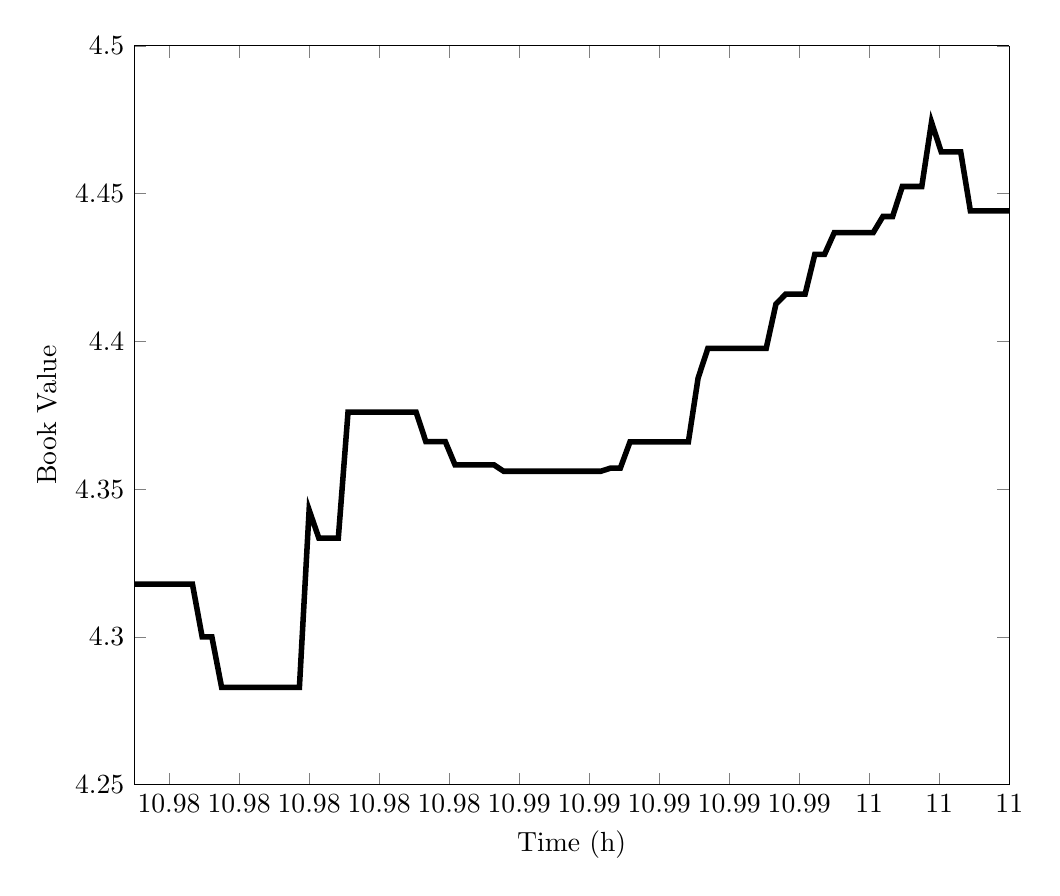
\begin{tikzpicture}

\begin{axis}[%
width=4.376in,
height=3.694in,
at={(1.256in,0.622in)},
scale only axis,
separate axis lines,
every outer x axis line/.append style={black},
every x tick label/.append style={font=\color{black}},
xmin=10.975,
xmax=11,
xlabel={Time (h)},
every outer y axis line/.append style={black},
every y tick label/.append style={font=\color{black}},
ymin=4.25,
ymax=4.5,
ylabel={Book Value},
axis background/.style={fill=white}
]
\addplot [color=black,solid,line width=2.0pt,forget plot]
  table[row sep=crcr]{%
10.975	4.31785157278387\\
10.9752777777778	4.31785157278387\\
10.9755555555556	4.31785157278387\\
10.9758333333333	4.31785157278387\\
10.9761111111111	4.31785157278387\\
10.9763888888889	4.31785157278387\\
10.9766666666667	4.31785157278387\\
10.9769444444444	4.29997516867812\\
10.9772222222222	4.29997516867812\\
10.9775	4.28292312893899\\
10.9777777777778	4.28292312893899\\
10.9780555555556	4.28292312893899\\
10.9783333333333	4.28292312893899\\
10.9786111111111	4.28292312893899\\
10.9788888888889	4.28292312893899\\
10.9791666666667	4.28292312893899\\
10.9794444444444	4.28292312893899\\
10.9797222222222	4.28292312893899\\
10.98	4.34292312893902\\
10.9802777777778	4.33340832904011\\
10.9805555555556	4.33340832904011\\
10.9808333333333	4.33340832904011\\
10.9811111111111	4.3760591839511\\
10.9813888888889	4.3760591839511\\
10.9816666666667	4.3760591839511\\
10.9819444444444	4.3760591839511\\
10.9822222222222	4.3760591839511\\
10.9825	4.3760591839511\\
10.9827777777778	4.3760591839511\\
10.9830555555556	4.3760591839511\\
10.9833333333333	4.36609262500156\\
10.9836111111111	4.36609262500156\\
10.9838888888889	4.36609262500156\\
10.9841666666667	4.3582162208958\\
10.9844444444444	4.3582162208958\\
10.9847222222222	4.3582162208958\\
10.985	4.3582162208958\\
10.9852777777778	4.3582162208958\\
10.9855555555556	4.35604079488735\\
10.9858333333333	4.35604079488735\\
10.9861111111111	4.35604079488735\\
10.9863888888889	4.35604079488735\\
10.9866666666667	4.35604079488735\\
10.9869444444444	4.35604079488735\\
10.9872222222222	4.35604079488735\\
10.9875	4.35604079488735\\
10.9877777777778	4.35604079488735\\
10.9880555555556	4.35604079488735\\
10.9883333333333	4.35604079488735\\
10.9886111111111	4.35709178725898\\
10.9888888888889	4.35709178725898\\
10.9891666666667	4.36600984698629\\
10.9894444444444	4.36600984698629\\
10.9897222222222	4.36600984698629\\
10.99	4.36600984698629\\
10.9902777777778	4.36600984698629\\
10.9905555555556	4.36600984698629\\
10.9908333333333	4.36600984698629\\
10.9911111111111	4.38759025344325\\
10.9913888888889	4.39759025344324\\
10.9916666666667	4.39759025344324\\
10.9919444444444	4.39759025344324\\
10.9922222222222	4.39759025344324\\
10.9925	4.39759025344324\\
10.9927777777778	4.39759025344324\\
10.9930555555556	4.39759025344324\\
10.9933333333333	4.4125677800173\\
10.9936111111111	4.41595535917614\\
10.9938888888889	4.41595535917614\\
10.9941666666667	4.41595535917614\\
10.9944444444444	4.42941120110194\\
10.9947222222222	4.42941120110194\\
10.995	4.43675598564101\\
10.9952777777778	4.43675598564101\\
10.9955555555556	4.43675598564101\\
10.9958333333333	4.43675598564101\\
10.9961111111111	4.43675598564101\\
10.9963888888889	4.44223960795387\\
10.9966666666667	4.44223960795387\\
10.9969444444444	4.45239406791461\\
10.9972222222222	4.45239406791461\\
10.9975	4.45239406791461\\
10.9977777777778	4.47413731127108\\
10.9980555555556	4.46413731127109\\
10.9983333333333	4.46413731127109\\
10.9986111111111	4.46413731127109\\
10.9988888888889	4.44413731127105\\
10.9991666666667	4.44413731127105\\
10.9994444444444	4.44413731127105\\
10.9997222222222	4.44413731127105\\
11	4.44413731127105\\
};
\end{axis}
\end{tikzpicture}%%
  \hspace{1.5cm}%
  %\tikzsetnextfilename{samplepath_dscr_nFPC_inventory}%
  % This file was created by matlab2tikz.
%
%The latest updates can be retrieved from
%  http://www.mathworks.com/matlabcentral/fileexchange/22022-matlab2tikz-matlab2tikz
%where you can also make suggestions and rate matlab2tikz.
%
\begin{tikzpicture}[trim axis left, trim axis right]

\begin{axis}[%
width=\figurewidth,
height=\figureheight,
at={(0\figurewidth,0\figureheight)},
scale only axis,
separate axis lines,
every outer x axis line/.append style={black},
every x tick label/.append style={font=\color{black}},
xtick = {10.97,10.98,10.99,11},
xmin=10.975,
xmax=11,
ylabel near ticks,
yticklabel pos=right,
every outer y axis line/.append style={black},
every y tick label/.append style={font=\color{black}},
ymin=5,
ymax=11,
axis background/.style={fill=white}
]
\addplot [color=black,solid,line width=2.0pt,forget plot]
  table[row sep=crcr]{%
10.975	6\\
10.9752777777778	6\\
10.9755555555556	6\\
10.9758333333333	6\\
10.9761111111111	6\\
10.9763888888889	6\\
10.9766666666667	6\\
10.9769444444444	7\\
10.9772222222222	7\\
10.9775	8\\
10.9777777777778	8\\
10.9780555555556	8\\
10.9783333333333	8\\
10.9786111111111	8\\
10.9788888888889	8\\
10.9791666666667	8\\
10.9794444444444	8\\
10.9797222222222	8\\
10.98	5\\
10.9802777777778	6\\
10.9805555555556	6\\
10.9808333333333	6\\
10.9811111111111	5\\
10.9813888888889	5\\
10.9816666666667	5\\
10.9819444444444	5\\
10.9822222222222	5\\
10.9825	5\\
10.9827777777778	5\\
10.9830555555556	5\\
10.9833333333333	6\\
10.9836111111111	6\\
10.9838888888889	6\\
10.9841666666667	7\\
10.9844444444444	7\\
10.9847222222222	7\\
10.985	7\\
10.9852777777778	7\\
10.9855555555556	8\\
10.9858333333333	8\\
10.9861111111111	8\\
10.9863888888889	8\\
10.9866666666667	8\\
10.9869444444444	8\\
10.9872222222222	8\\
10.9875	8\\
10.9877777777778	8\\
10.9880555555556	9\\
10.9883333333333	9\\
10.9886111111111	10\\
10.9888888888889	10\\
10.9891666666667	11\\
10.9894444444444	11\\
10.9897222222222	11\\
10.99	11\\
10.9902777777778	11\\
10.9905555555556	11\\
10.9908333333333	11\\
10.9911111111111	8\\
10.9913888888889	7\\
10.9916666666667	7\\
10.9919444444444	7\\
10.9922222222222	7\\
10.9925	7\\
10.9927777777778	7\\
10.9930555555556	7\\
10.9933333333333	8\\
10.9936111111111	7\\
10.9938888888889	7\\
10.9941666666667	7\\
10.9944444444444	6\\
10.9947222222222	6\\
10.995	7\\
10.9952777777778	7\\
10.9955555555556	7\\
10.9958333333333	7\\
10.9961111111111	7\\
10.9963888888889	8\\
10.9966666666667	8\\
10.9969444444444	9\\
10.9972222222222	9\\
10.9975	9\\
10.9977777777778	8\\
10.9980555555556	9\\
10.9983333333333	9\\
10.9986111111111	9\\
10.9988888888889	10\\
10.9991666666667	10\\
10.9994444444444	10\\
10.9997222222222	10\\
11	10\\
};
\end{axis}
\end{tikzpicture}%
%
  \caption{Discrete Time w/ nFPC}%
\end{subfigure}\\%
\leavevmode\smash{\makebox[0pt]{\hspace{-4em}% HORIZONTAL POSITION           
  \rotatebox[origin=l]{90}{\hspace{20em}% VERTICAL POSITION
    Profit and Loss (P\&L) (\$)}%
}}\smash{\makebox[0pt]{\hspace{2.05\linewidth}% HORIZONTAL POSITION           
  \rotatebox[origin=l]{90}{\hspace{23em}% VERTICAL POSITION
	Inventory}%
}}\hspace{0pt plus 1filll}\null%

Time (h)

\vspace{1cm}%
  \caption[Comparison of P\&L and inventory on the sample path]{Profit and loss and inventory levels resulting from each of the stochastic optimal control strategies, corresponding to the sample paths in \autoref{fig:samplepath_paths}.}\label{fig:samplepath_pnl_inv}%
\end{figure}

\end{document}